%======================================================================
\chapter{Valence Bond Entanglement Entropy}
%======================================================================


\section{One Dimensional Systems}


\begin{figure} {
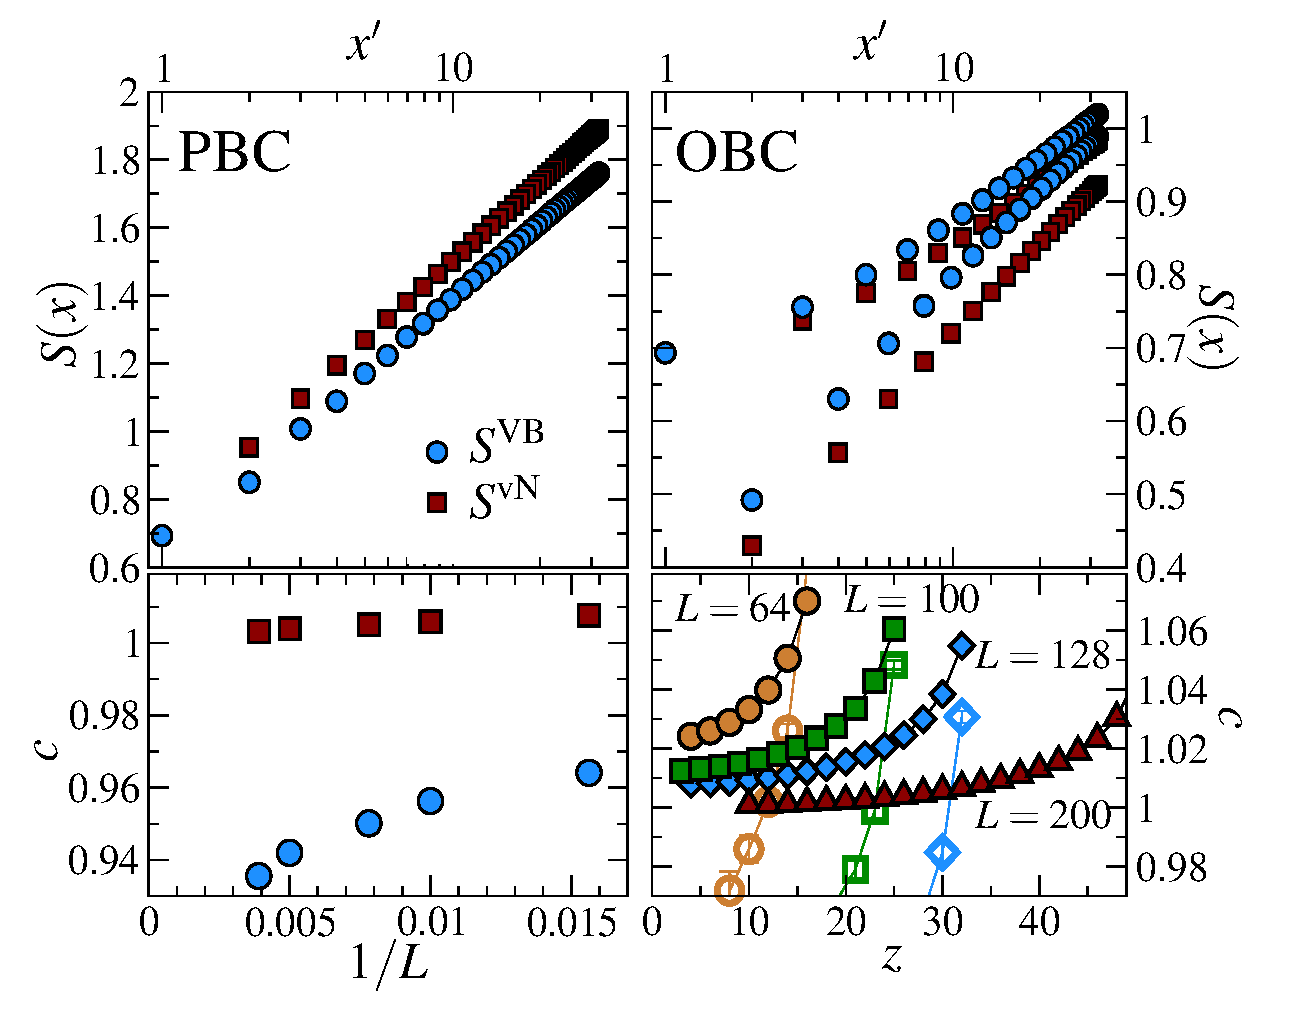
\includegraphics[width=6.5in]{./figures/paper1/figure1/4-panelFIG1.eps} 
\centering
\caption[1D Results for VB EE and von Neumann EE]{
{\color{red}
Entanglement entropies for a 1D Heisenberg chain with PBC and OBC. Upper
panels show the entropies as a function of the conformal distance $x'  = (L/\pi)\sin (\pi x/L)$ for
100-site chains.  Lower plots show the central
charge $c$, obtained by fitting the numerical data to the CFT result, for
several $L$.  For PBC, $c$ is calculated with the two smallest $x'$ points
removed.  For OBC, the fits depend on the number of sites included, $z$,
which we systematically decrease by removing $x'$ data points from the
{\it outside} ends of the chain.  $c$ is shown for $S^{\rm vN}$
(closed symbols) and $S^{\rm VB}$ (open symbols) for system sizes $L=64$
(circles), $L=100$ (squares), $L=128$ (diamonds), and $L=200$ (triangles)
\label{1D}}
} }
\end{figure}



\section{Approaching Two Dimensions}

\begin{figure} { 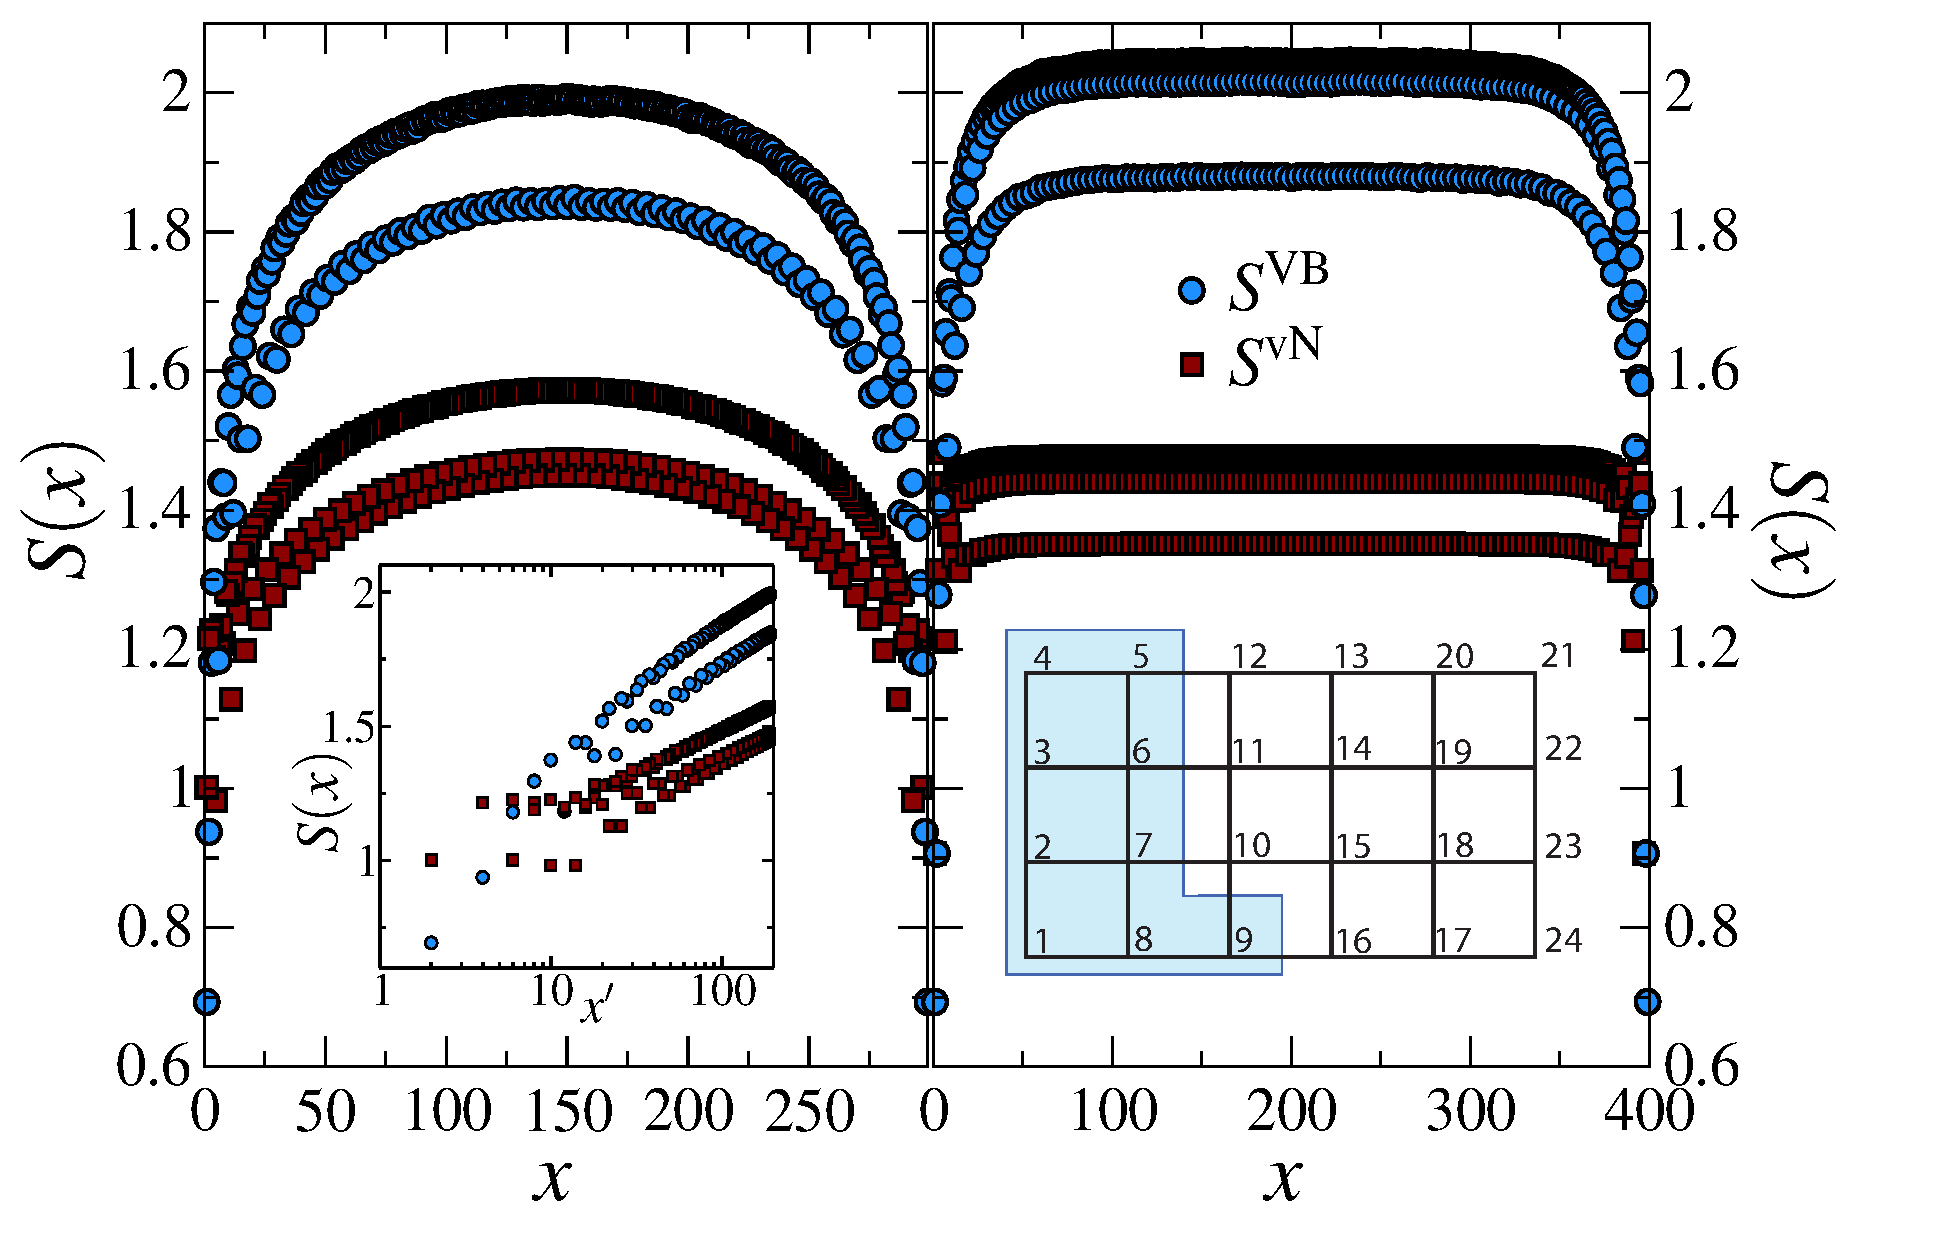
\includegraphics[width=6.5in]{./figures/paper1/figure23new/fig23NEW.eps}
\caption[EEs for 3- \& 4-leg ladders]{
{\color{red}
Entanglement entropies for 3-leg (left)
and 4-leg (right) ladder systems with OBC and 100 sites per leg.  For
odd-leg ladders, $S(x)\propto\ln(x')$.  The left
inset shows $S(x)$ as a function of the conformal distance, $x'$, on a log
scale. For even-leg ladders, $S(x\gtrsim\xi)= {\rm const}.$
The right inset shows the site indexing used for multi-leg ladders where the
bipartition A is shaded and labeled by $x=9$. 
}
 \label{ladder} }} 
 \end{figure}

\section{The Area Law}

\begin{figure} { \includegraphics[width=6.5in]{./figures/paper1/figure4/fig4.eps}
 \caption[Area Law in 2D Heis model]{
 {\color{red} Entanglement entropies divided by $N$,  for $N$-leg Heisenberg
(filled symbols) and free-fermion (open diamonds) ladders, taken such that
the region A includes $2N^2$ sites.  
For the Heisenberg model and large $N$, $S^{\rm VB}\propto N \ln N$,
whereas $S^{\rm vN}\propto N$.  
Data for free fermions, $S^{\rm vN}_{\rm ff}\propto N \ln N$,  are shown for comparison.
We show data for ladders with length (sites per leg) $L =100$ and
%ladders with length proportional to the number of legs 
$L=4N$.  
}
\label{zigzag}}} 
\end{figure}
